\documentclass[12pt,fleqn]{article}\usepackage{../common}
\begin{document}
Ders 15

Konumuz cok, cok buyuk ve seyrek matrisler uzerinden $Ax = b$ cozumu. Cok
buyuk boyutlarda $A$'nin tersini almak pahali bir islem olacaktir. Standart
teknik Gauss Eliminiasyon teknigi de yuksek boyutlarda pahali bir islem
olur. Pahali olmayan islem nedir? $A$'yi bir vektor ile carpmaktir
mesela. Bu islemin nasil devreye girecegini gorecegiz.

Genel ismiyle daha hizli olacak genel kategori ozyineli (iterative)
metotlardir. Bu yontemlerde en iyi cevaba erismeyiz, ama yeterince
yaklasiriz, ve daha onemlisi bu isi cok hizli bir sekilde
yapabiliriz. Bu metotlarda iyi bir onkosullandirici (preconditioner)
matris $P$'yi secmek onemlidir. $P$, $A$'yi temel alan ve bazi islemleri
kolaylastiran bir yapi olacaktir. 

Ozyineli tekniklerden en iyi bilinenlerden biri eslenik gradyan
teknigidir. Bu yontem icin $A$'nin simetrik, pozitif kesin olmasi gerekir.

Ozyineli metotlarda bir baslangic $x_0$ degeri vardir, ve oradan $x_{k+1}$
elde edilir. Lineer metotlar icin baslangicin nerede oldugu onemli
degildir, sifirda bile baslanabilir. Gayrilineer (nonlinear), ``Newton''
metotlarinda sonuca yakin bir yerde olmak onemlidir, bunun icin ugrasilir.

Cozmek istedigimiz 

\[ Ax = b \]

Bunu soyle de yazabilirim 

\[ x = x - Ax + b \]

\[ x = (I - A)x + b \]

Simdi bu denklemi alip sag tarafi ``eski'' sol tarafi ``yeni'' olarak
temsil edersek,

\[ x_{k+1} = (I - A)x_k + b \]

elde ederiz. Bu onkosulsuz, basit bir ozyinelemedir. Onkosul $P$ istersek,

\[ Ax = b \]

\[ 0 = -Ax + b \]

\[ Px = Px - Ax + b \]

\[ Px = (P -A)x + b \]

\[ Px_{k+1} =  (P - A)x_k + b \]

Eger $P = A$ olsaydi, o zaman direk eski denklemi cozuyor olurduk.  
Biz $P
\approx A$ dedik, ``yakin ama ayni olmayan bir $P$'' istiyoruz,
ozellikle. Bu $P$'nin islerimizi kolaylastiracagini umuyoruz cunku.

Bazi $P$ ornekleri sunlardir: Jacobi $A$'nin sadece caprazindaki degerleri
alip $P$'ye koyar. Gauss-Seidel yaklasimi [1], hem caprazi, hem alt ucgensel
(lower triangular) kismi alip $P$'ye koyar.

Diger yaklasimlar fazla rahatlatma (overrelaxation), ve tamamlanmmamis
(incomplete) LU gibi yaklasimlar. Ben ustlisans yaparken bu son iki yontem
Jacobi, Gauss-Seidel'den bir adim ileri gitme yonundeki denemelerin
baslangiciydi. 

Peki $x$'lerin dogru cevaba erisip erismedigini nereden anlariz? Hata
hesabi icin bir formule ihtiyacim var. Alttaki formullerde 2. formulu
1. formulden cikartirsam, ve $e_k = x - x_k$ ise

\[ x_{k+1} = (I - A)x_k + b \]

\[ x_k = (I - A)x + b \]

Sunu elde ederim,

\[ Pe_{k+1} = (P-A)e_k \]

Iki tarafi $P^{-1}$ ile carparsam,

\[ e_{k+1} = (I-P^{-1}A)e_k = Me_k\]

O zaman hata hesabi icin her ozyineleme adiminda ustteki hesabi
yaparim. Parantez icindeki buyuk ifadeye $M$ ismi verdim, buna ozyineleme
matrisi de diyebiliriz. 

Degerlere yakinda bakarsak, $P$'nin $A$'ya yakin olmasini istiyoruz
demistik, o zaman $P^{-1}A$, $I$'ya yakin olacaktir, ve bu $I$'ya yakin
olan sey $I$'dan cikartilinca sonuc sifira yakin olacaktir. Hatanin ufak
olmasini istedigimize gore bu mantikli. 

Her adimda $M$ ile carptigimiza gore, 

\[ e_k = M^k e_0 \]

Ustteki sifira gider mi? Giderse ne kadar hizli gider? Bunun olmasi icin
$M$'nin hangi ogesine bakmak gerekir? En buyuk ozdegerine bakmak
gerekir. Genel olarak sunu soyleyebiliriz, her $|\lambda(M)| < 1$ olmasi
gerekir. Notasyonel olarak en buyuk ozdeger $\rho(M)$'dir, $|\rho(M)|$ ise
spektral yaricapi (spectral radius) olarak adlandirilir.

Bazi ornekler

\[ K = A = 
\left[\begin{array}{rrrr}
2 & -1 && \\
& 2 & -1 & \\
&&& \\
&& -1 & 2 \\
\end{array}\right]
 \]

Ozdegerler $\lambda_j(A) = 2 - 2 \cos\theta_j$

$P_{Jacobi} = 2I$

\[ M = I-P^{-1}A  \]

Sonuc

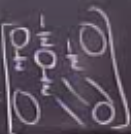
\includegraphics[height=2cm]{15_1.png}

Yani $P^{-1} = 1/2$

\[ M = I-\frac{ 1}{2}A  \]

\[ \lambda_j(M) = 1 - \frac{ 1}{2}\lambda_j(A) = \cos \frac{ j\pi}{N+1}\]

O zaman yaklasiksallama olacak. En buyuk ozdeger

\[ \rho = \cos \frac{ \pi}{N+1} \]

Eger her dongude bir seyleri grafiklemek istesem, neyi secerdim? Her
dongudeki hatayi, ``artigi (residual)'' grafikleyebilirdim. Tam denklem

\[ Ax = b \]

$Ax_k$ gercege ``yakin'', o zaman artik deger $r$ bu ikisi arasindaki fark
olabilir, 

\[ r = Ax - Ax_k \]

\[ r = Ae_k \]

[hata grafikleme atlandi]

Ornek Jacobi kodlari

\lstinputlisting[language=Python]{jacobi.py}

\lstinputlisting[language=Python]{jacobi2.py}

Bu kodlarin ikisi de ozyineli Jacobi hesabi yapiyor. Birincisi her dongude 
\verb!solve! islemi yapiyor. Fakat daha once belirttigimiz gibi, her
dongude carpim islemi yapmak cok daha optimal olur. Ikinci kod [2]

\[ Px_{k+1} =  (P - A)x_k + b \]

islemini iki parcaya ayirmis, $P,P-A$ ve $P,b$ sistemlerini ayri ayri
cozerek, dongu icinde $Jx + c$ ile sadece carpma ve toplama kullanmayi
basarmis. Bu parcalamanin yapilabilmesinin sebebi tabii ki bir lineer
sistemle calisiyor olmamiz. Cok akillica bir teknik. 

Kaynaklar

[1] Ilginc bir tarihi anektod, Gauss Eliminasyon yontemini kesfeden bizzat
Gauss'un kendisi bile bu yontemi kullanmak istememisti, buyuk matrislerde
eliminasyon isinin ozellikle hesabin elle yapildigi eski yilllarda cok
kulfet getiriyordu. Ozyineli ilk metotlardan Gauss-Seidel teknigi Gauss'u
cok memnun etti, ve kendi hesaplarinda bu teknigi kullandi.

[2] http://www.math.umn.edu/~olver/matlab.html










\end{document}
